\documentclass[10pt,twoside,slovak,a4paper]{article}

\usepackage[slovak]{babel}
%\usepackage[T1]{fontenc}
\usepackage[IL2]{fontenc} % lepšia sadzba písmena Ľ než v T1
\usepackage[utf8]{inputenc}
\usepackage{graphicx}
\usepackage{url} % príkaz \url na formátovanie URL
\usepackage{hyperref} % odkazy v texte budú aktívne (pri niektorých triedach dokumentov spôsobuje posun textu)

\usepackage{cite}
%\usepackage{times}

\pagestyle{headings}

\title{Názov\thanks{Semestrálny projekt v predmete Metódy inžinierskej práce, ak. rok 2015/16, vedenie: Meno Priezvisko}} % meno a priezvisko vyučujúceho na cvičeniach

\author{Meno Priezvisko\\[2pt]
	{\small Slovenská technická univerzita v Bratislave}\\
	{\small Fakulta informatiky a informačných technológií}\\
	{\small \texttt{...@stuba.sk}}
	}

\date{\small 30. september 2015} % upravte



\begin{document}

\maketitle

\begin{abstract}
\ldots
\end{abstract}

\usepackage{graphicx}
\usepackage{pdfpages}
\begin{figure}
 \centering 
 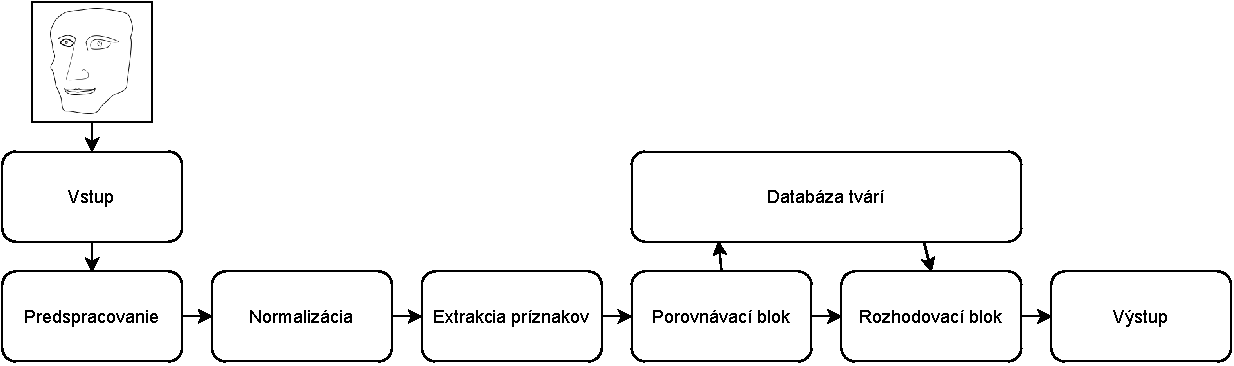
\includepdf[pages=-]{Diagram0crop.drawio.pdf}
\end{figure}